\documentclass[10pt]{beamer}

\usetheme{m}

\usepackage{booktabs}
\usepackage[scale=2]{ccicons}

\usepackage{multicol}

\usepackage{pgfplots}
\usepgfplotslibrary{dateplot}

\usepackage{upgreek}

 
\newtheorem{examplenegative}{exampleblock}
\newenvironment<>{examplenegative}[1]{%
  \setbeamercolor{block title example}{fg=red}%
  \begin{exampleblock}#2{#1}}{\end{exampleblock}}


\setbeamercovered{invisible}

%Notes on laptop but not on presentation
%\usepackage{pgfpages}
%\setbeameroption{show notes}
%\setbeameroption{show notes on second screen=right}
%\setbeameroption{show notes on second screen}

\usepackage[]{algorithm2e}
\makeatletter
\usepackage{color}
\definecolor{editorLightGray}{cmyk}{0.05, 0.05, 0.05, 0.1}
\definecolor{editorGray}{cmyk}{0.6, 0.55, 0.55, 0.2}
\definecolor{editorPurple}{cmyk}{0.5, 1, 0, 0}
\definecolor{editorWhite}{cmyk}{0, 0, 0, 0}
\definecolor{editorBlack}{cmyk}{1, 1, 1, 1}
\definecolor{editorOrange}{cmyk}{0, 0.8, 1, 0}
\definecolor{editorBlue}{cmyk}{1, 0.6, 0, 0}
\definecolor{editorPink}{cmyk}{0, 1, 0, 0}
\usepackage{upquote}
\usepackage{listings}
% CSS
\lstdefinelanguage{CSS}{
  keywords={color,background-image:,margin,padding,font,weight,display,position,top,left,right,bottom,list,style,border,size,space,min,width, transition:, transform:, transition-property, transition-duration, transition-timing-function, background:, color:, background-color:}, 
  sensitive=true,
  morecomment=[l]{//},
  morecomment=[s]{/*}{*/},
  morestring=[b]',
  morestring=[b]",
  alsoletter={:},
  alsodigit={-}
}

% JavaScript
\lstdefinelanguage{JavaScript}{
  morekeywords={typeof, new, true, false, catch, function, return, null, catch, switch, var, if, in, while, do, else, case, break},
  morecomment=[s]{/*}{*/},
  morecomment=[l]//,
  morestring=[b]",
  morestring=[b]'
}

\lstdefinelanguage{HTML5}{
  language=html,
  sensitive=true,   
  alsoletter={<>=-+},   
  morecomment=[s]{<!-}{-->},
  tag=[s],
  otherkeywords={
  % General
  % >,
  % Standard tags
    <!DOCTYPE,
  </html, <html, <head, <title, </title, <style, </style, <link, </head, <meta, />,
    % body
    </body, <body,
    % Divs
    </div, <div, </div>, 
    % Paragraphs
    </p, <p, </p>,
    % scripts
    </script, <script,
  % More tags...
  <canvas, /canvas>, <svg, <rect, <animateTransform, </rect>, </svg>, <video, <source, <iframe, </iframe>, </video>, <image, </image>
  },
  ndkeywords={=,
  % General
  +=,
  % HTML attributes
   charset=, src=, id=, width=, height=, style=, type=, rel=, href=,
  % SVG attributes
  fill=, attributeName=, begin=, dur=, from=, to=, poster=, controls=, x=, y=, repeatCount=, xlink:href=,
  % CSS properties
  margin:, padding:, background-image:, border:, top:, left:, position:, width:, height:,
    % CSS3 properties
  transform:, -moz-transform:, -webkit-transform:,
  animation:, -webkit-animation:,
  transition:,  transition-duration:, transition-property:, transition-timing-function:,
  },
}



\makeatother


\title{App-udvikling}
\subtitle{5. Lektion}
\date{\today}
\author{Sune Sylvest Nilausen}
%\institute{Institute or miscellaneous information}
% \titlegraphic{\hfill\includegraphics[height=1.5cm]{logo/logo}}
\graphicspath{ {../} }

\begin{document}
%\setbeamertemplate{caption}{\raggedright\insertcaption\par}

\maketitle

\begin{frame}
  \frametitle{Indholdsfortegnelse}
  \setbeamertemplate{section in toc}[sections numbered]
  \tableofcontents[hideallsubsections]
\end{frame}
%Forhenværende lektioner gik ud på at lære de første trin i at designe et produkt.
%Altså at designe et app.

\section{Opsummering fra sidst}
\begin{frame}{Lille Quiz}
	\begin{itemize}
		\item \textbf{Hvad er en sketch?}
		\pause
		\begin{itemize}
			\item Ufærdig tegning
			\item Hjælpemiddel til at fange og udforske ideer
		\end{itemize}
		\item \textbf{Hvad er en prototype?}
		\pause
			\begin{itemize}
				\item En tidlig version af dit produkt
				\item Bruges til at teste og videreudvikle
			\end{itemize}
		\item \textbf{Hvad er en brugbarhedstest?}
		\pause
			\begin{itemize}
				\item En test til at finde designfejl
				\item Bruger et håndgribelig produkt til at få feedback
			\end{itemize}
	\end{itemize}

\end{frame}

\begin{frame}{Ideation}
		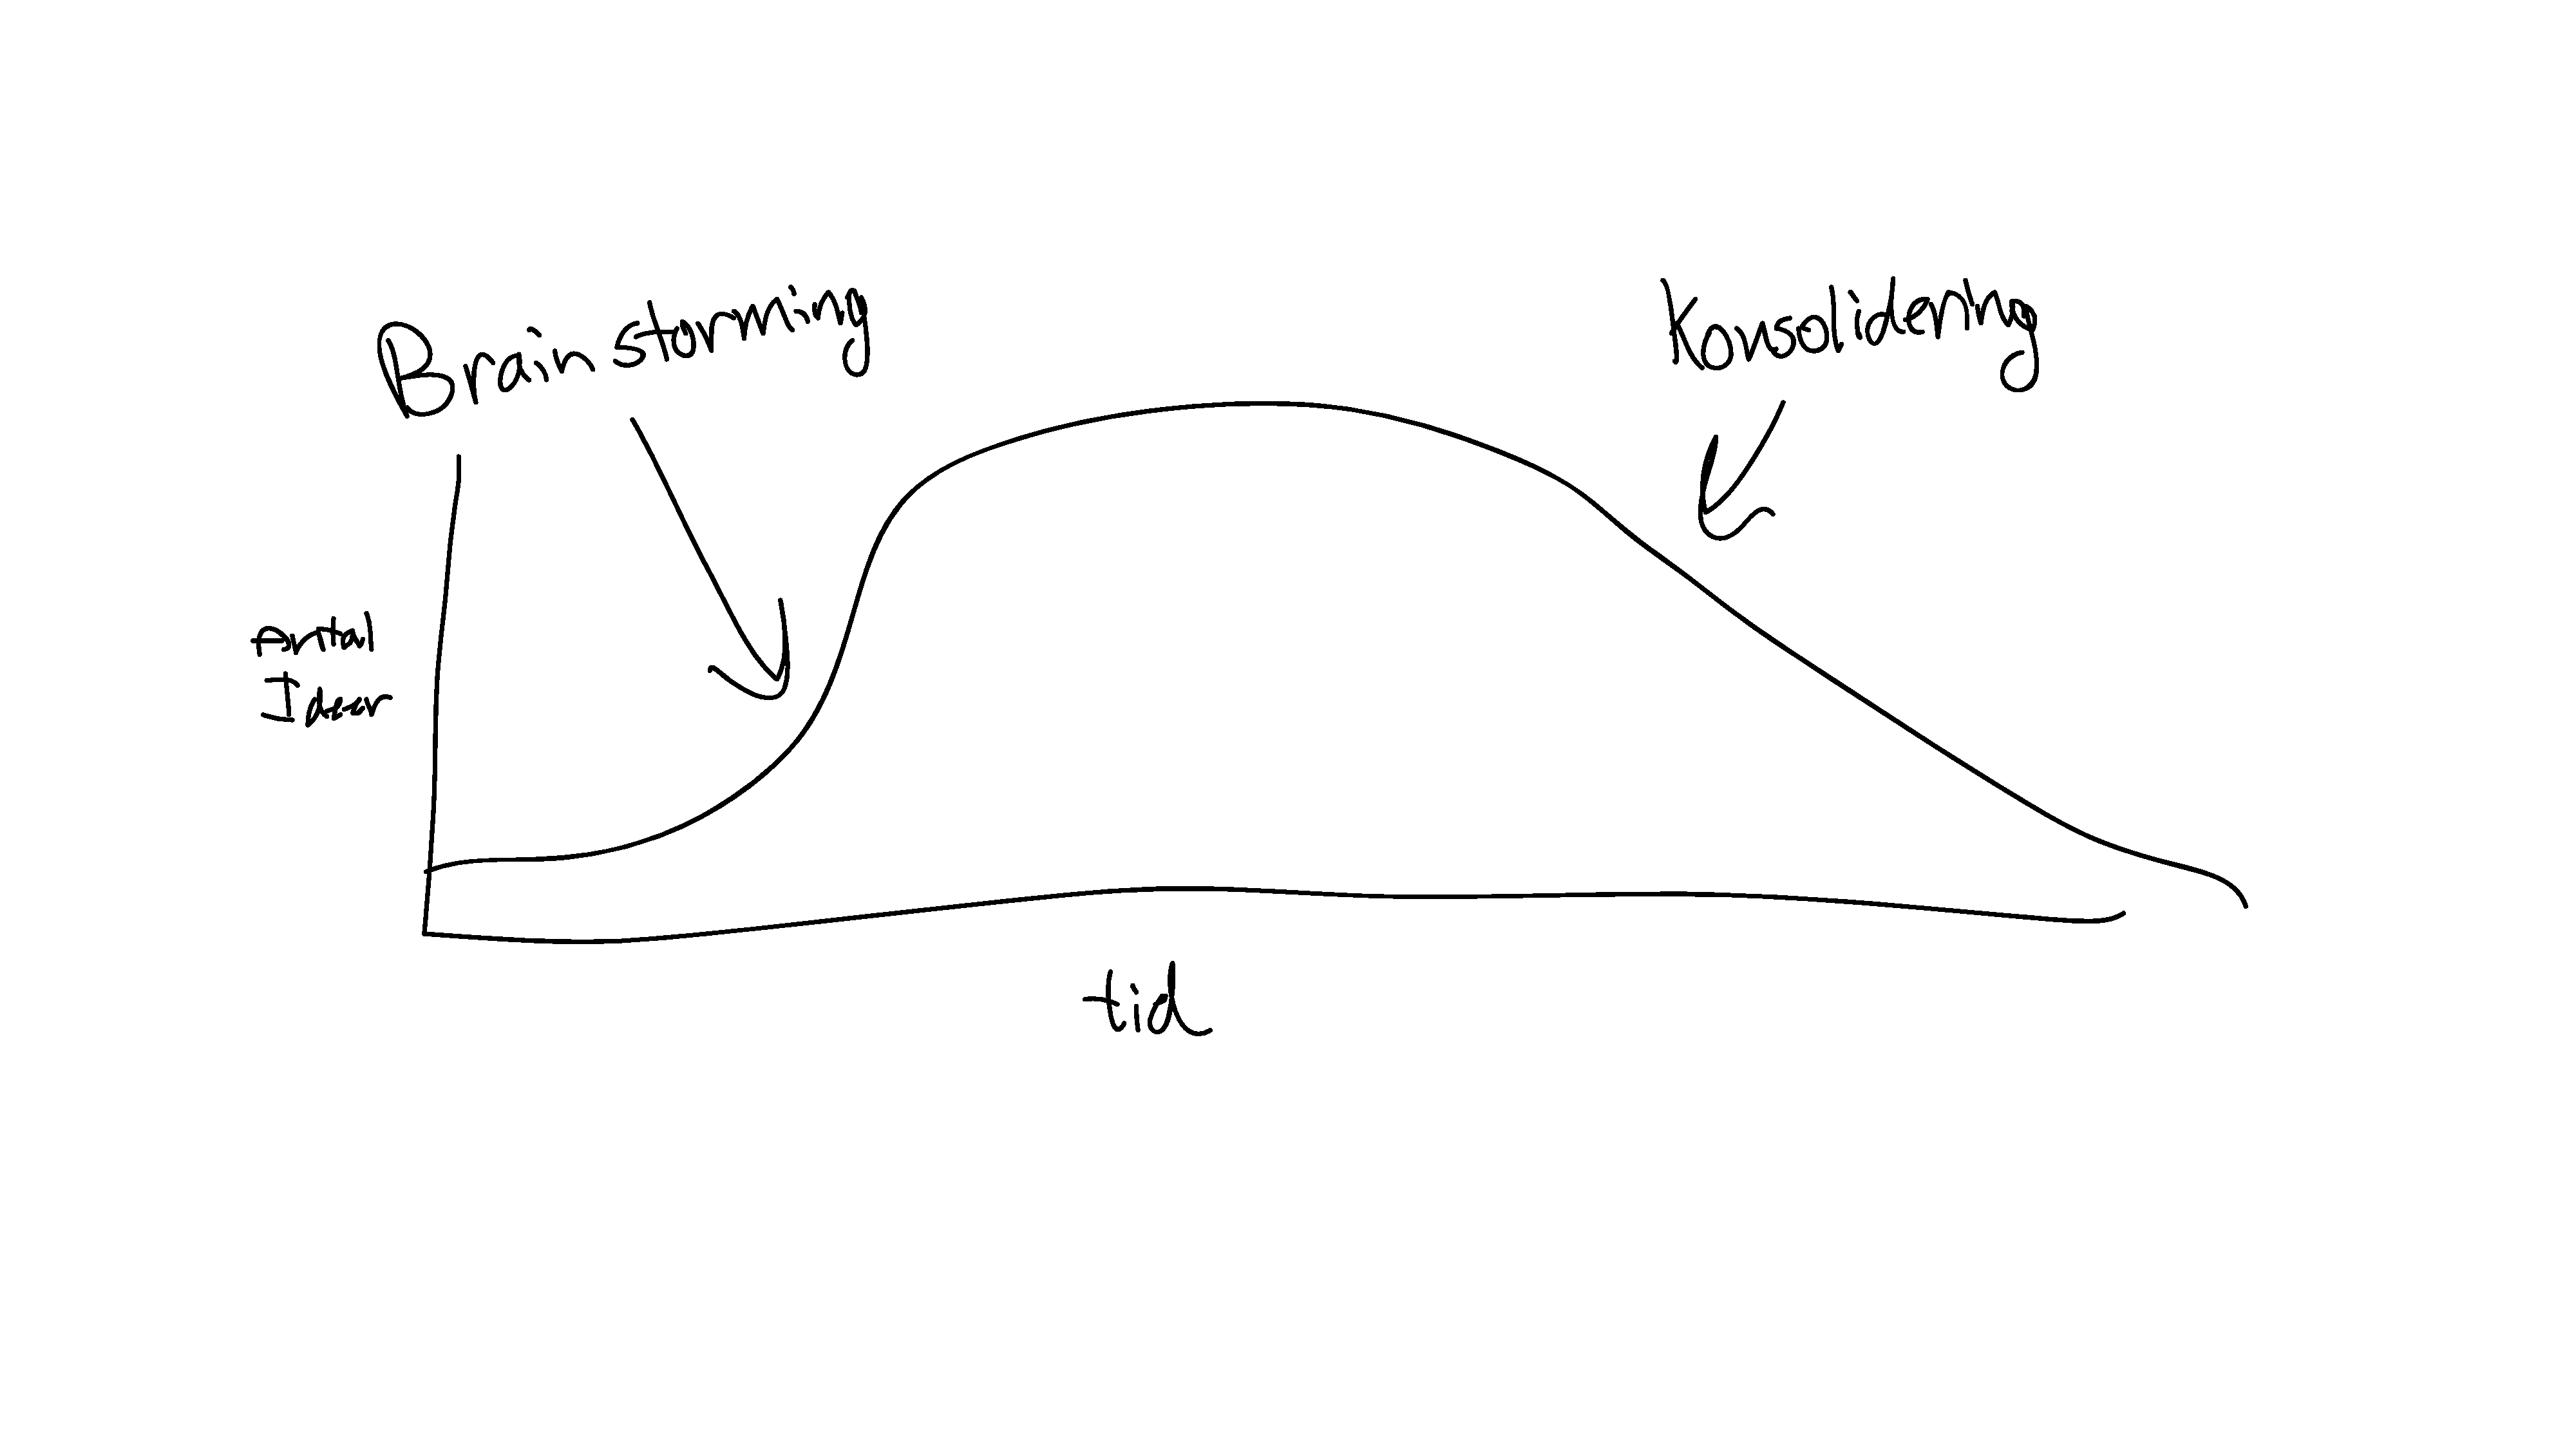
\includegraphics[scale=0.18]{img/ideation.pdf}
\end{frame}

\begin{frame}{Hvad er prototyper}
	\centering
	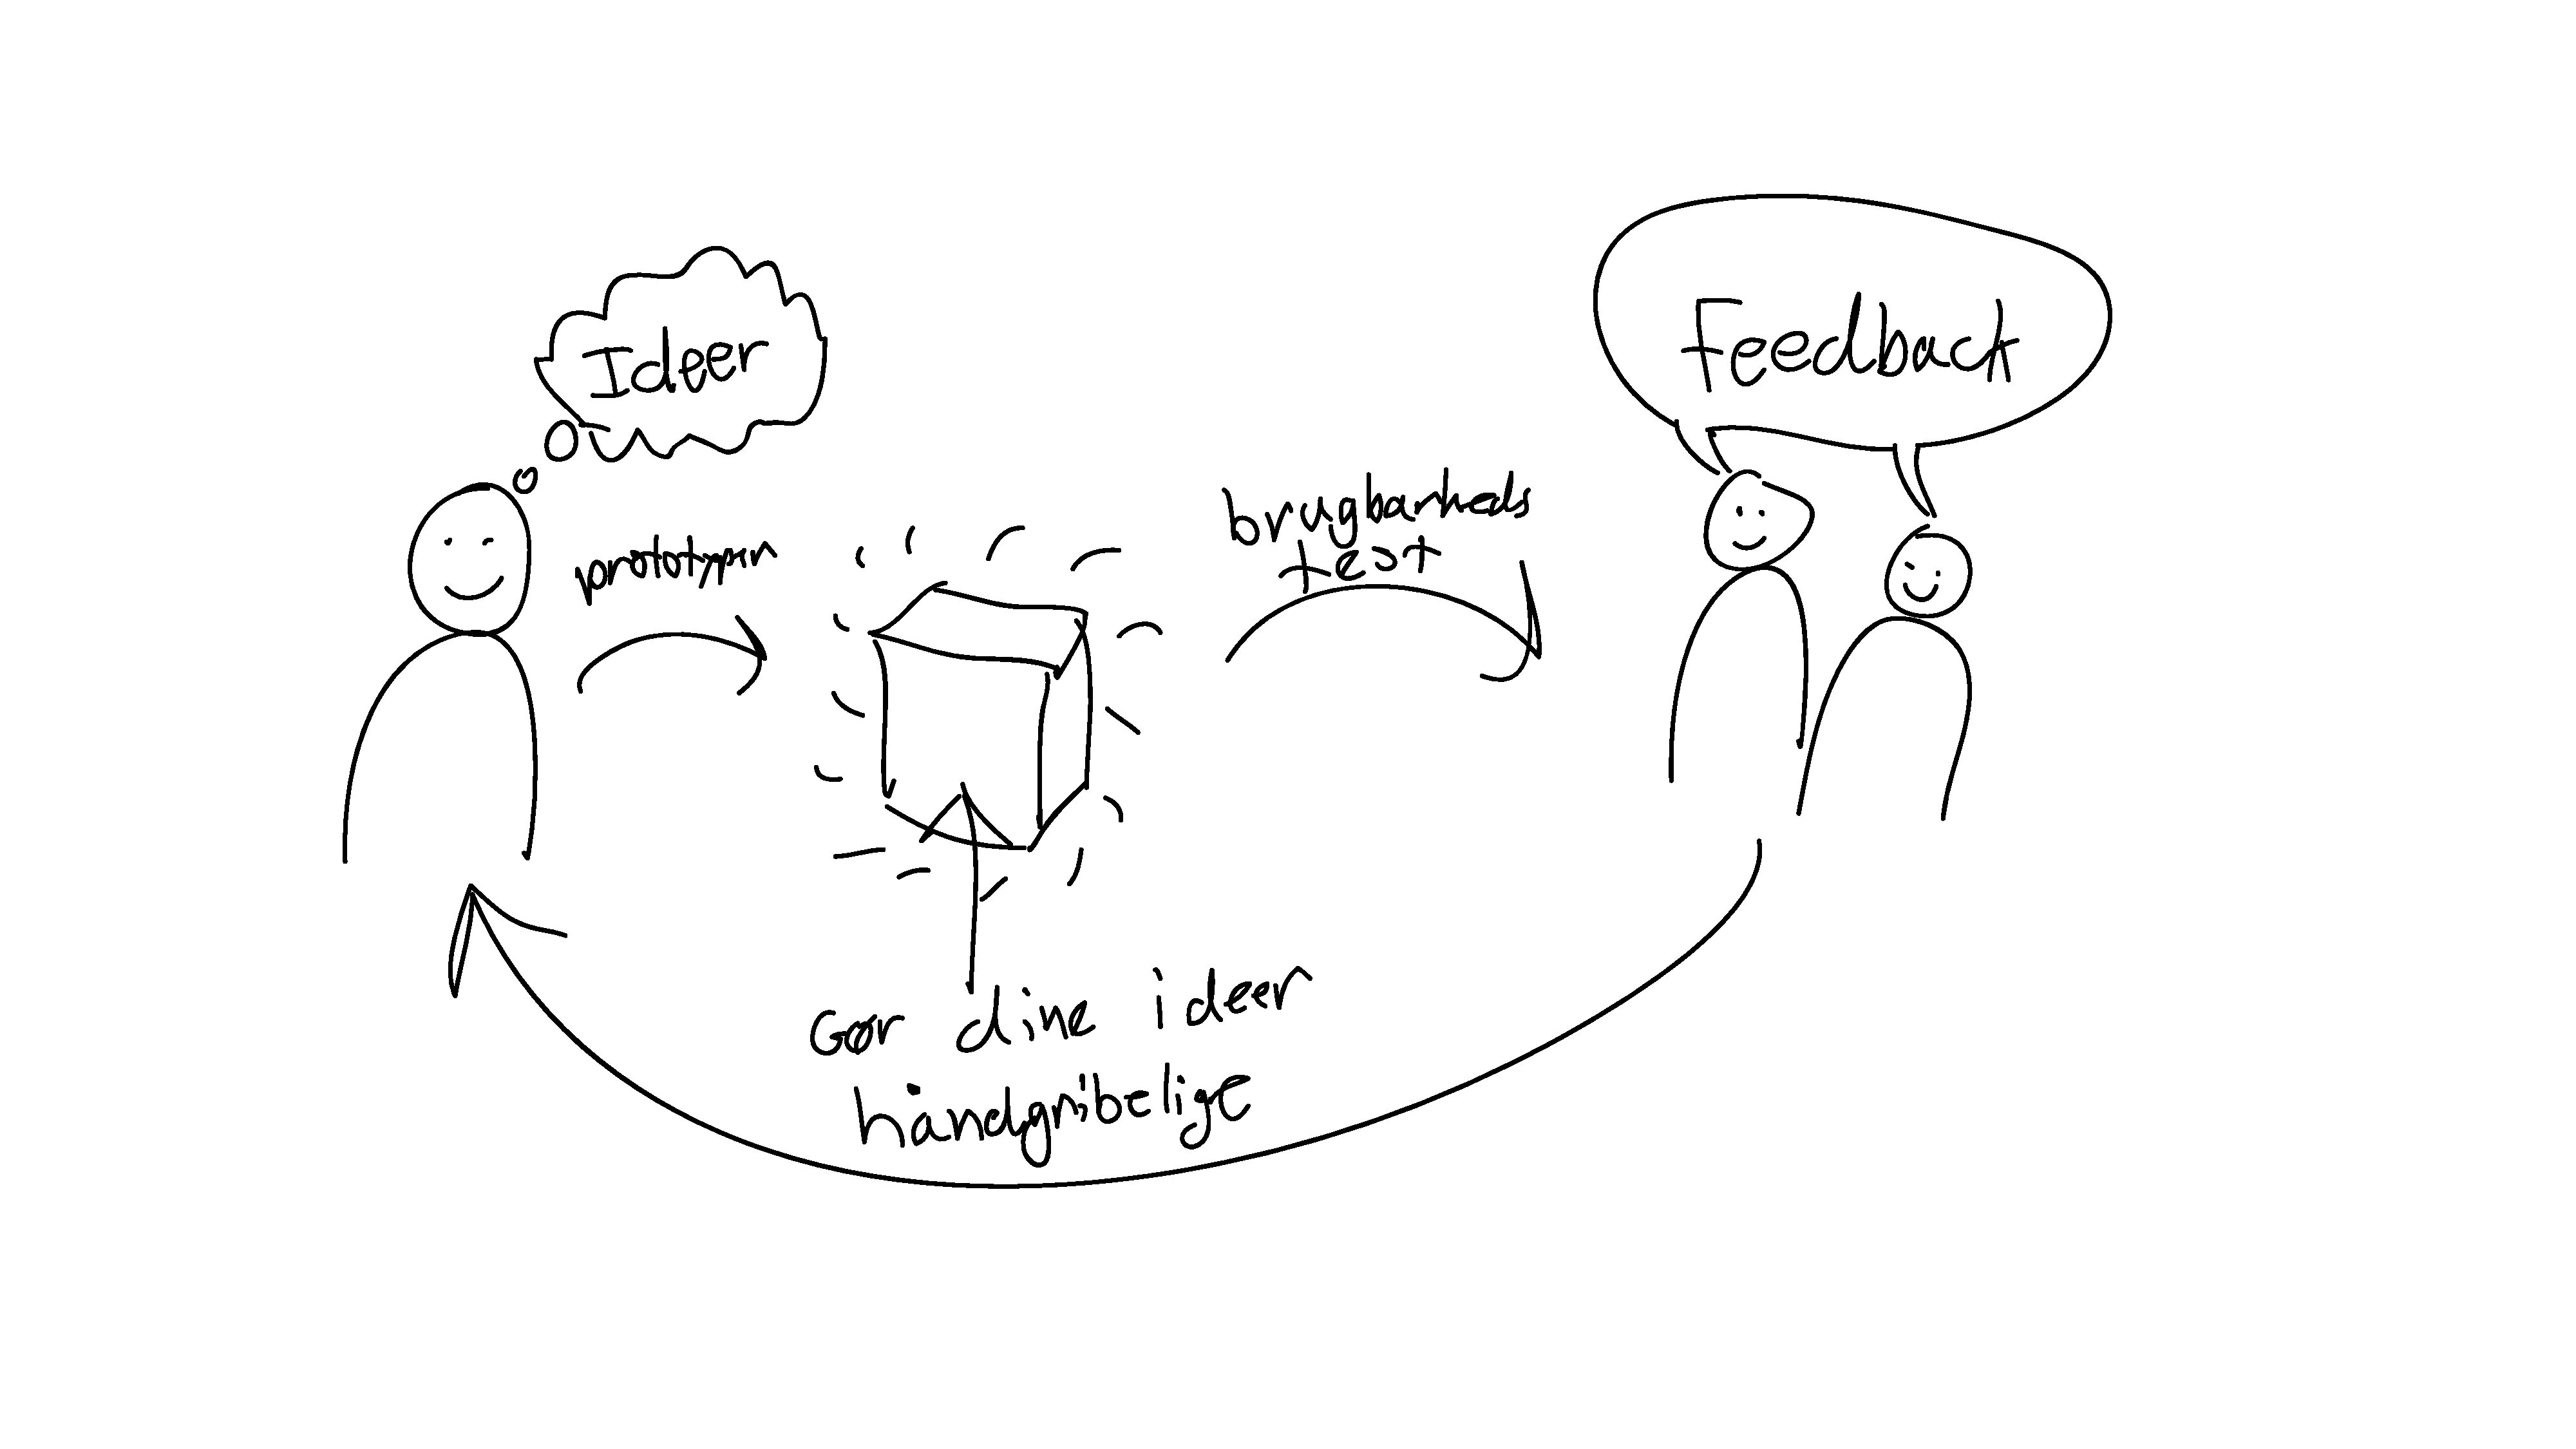
\includegraphics[scale=0.18]{img/prototypingloop.pdf}
\end{frame}

\begin{frame}{Brugbarhed / Usability}
		\includegraphics[width=\linewidth]{img/carusability.jpg}
\end{frame}


\section{HTML}

%Fremover skal vi begynde at lære om programmering og hvordan vi programmere et app.

\begin{frame}{Hvad er HTML?}
\begin{itemize}
	\item \textbf{H}yper \textbf{T}ext \textbf{M}arkup \textbf{L}anguage
	\item Den første af de 3 vigtigste web værktøjer.
	\item Bruges til at strukturere og definere indholdet på en hjemmeside.
\end{itemize}
\end{frame}

\begin{frame}[fragile]
 \frametitle{HTML Kode}

\lstset{
  language=html,
  tagstyle=\color{editorBlue},
  basicstyle={\small\ttfamily},
  identifierstyle=\color{editorOrange},
  keywordstyle=\color{editorPink},
  commentstyle=\color{editorGray},
  stringstyle=\color{editorPurple}
}
\begin{lstlisting}
<!DOCTYPE html>
<html>
  <body>
    <!-- Kommentar -->
    <div id="box">
      <p>Hello World</p>
      <h1>Overskrift type 1</h1>
      <h2>Overskrift type 2</h2>
      <img src="html5.png" width="250px" height="250px">
    </div>
    <div>Test</div>
  </body>
</html>
\end{lstlisting}
\end{frame}


\plain{
Øvelse:
http://www.w3schools.com/html/exercise.asp
 }
 
\section{CSS}

%Fremover skal vi begynde at lære om programmering og hvordan vi programmere et app.

\begin{frame}{Hvad er CSS?}
\begin{itemize}
	\item \textbf{C}ascading \textbf{S}tyle \textbf{S}heets.
	\item Den anden af de 3 vigtigste web værktøjer.
	\item Bestemmer hvordan HTML indholdet ser ud.
\end{itemize}
\end{frame}

\begin{frame}[fragile]
 \frametitle{CSS Kode}

\lstset{
  language=HTML5,
  alsolanguage=CSS,
  tagstyle=\color{editorBlue},
  basicstyle={\small\ttfamily},
  identifierstyle=\color{editorOrange},
  keywordstyle=\color{editorPink},
  commentstyle=\color{editorGray},
  stringstyle=\color{editorPurple}
}
\begin{lstlisting}
h1 { color: white;
background: orange;
border: 1px solid black;
}
body {background-color: white;
color: black;
border: 12px solid;
}
/* Kommentar */
\end{lstlisting}
\end{frame}



\plain{
Øvelse:
http://www.w3schools.com/css/exercise.asp
 }
 
\section{Javascript}

%Fremover skal vi begynde at lære om programmering og hvordan vi programmere et app.

\begin{frame}{Hvad er Javascript?}
	\begin{itemize}
		\item Et programmeringsprog.
		\item Den anden af de 3 vigtigste web værktøjer.
		\item Kører normalt kode på klient-siden til websider og mere.
	\end{itemize}
\end{frame}

\begin{frame}{Hvad er et Programmeringsprog?}
		\includegraphics[width=\linewidth]{img/programminglanguageslevels.jpg}
\end{frame}

\begin{frame}[fragile]
 \frametitle{Javascript Kode}

\lstset{
  language=JavaScript,
  tagstyle=\color{editorBlue},
  basicstyle={\small\ttfamily},
  identifierstyle=\color{editorOrange},
  keywordstyle=\color{editorPink},
  commentstyle=\color{editorGray},
  stringstyle=\color{editorPurple}
}
\begin{lstlisting}
// Dette er en kommentar

// Kan ændre på HTML
document.getElementById("demo").innerHTML = "Hello JavaScript";

// Siger "Hello World" med konsollen
console.log("Hello World!");
\end{lstlisting}
\end{frame}

\begin{frame}[fragile]
 \frametitle{JavaScript Variabler, Typer \& Operationer}

\lstset{
  language=JavaScript,
  tagstyle=\color{editorBlue},
  basicstyle={\small\ttfamily},
  identifierstyle=\color{editorOrange},
  keywordstyle=\color{editorPink},
  commentstyle=\color{editorGray},
  stringstyle=\color{editorPurple}
}
\begin{lstlisting}
//Variabler
var x;
x = 1;
var y = 2;

//Typer
var a = "En" //string
var b = 2.2 //tal
var d = true //boolean, kan også være false

//Matematiske operationer
var d = x+y;  // 1+2
var e = a + " To"  // svarer til "En To"
var f = 2*3;
var g = y/2;
var h = (1+2)*3;
var i = (true + true) * 5 // 10;
\end{lstlisting}
\end{frame}

\plain{
Øvelse:\\
Find nogle operationer hvor forskellige typer giver NaN
}
 
\begin{frame}[fragile]
\frametitle{JavaScript Kontrol Strukturer \& Sammenlignings Udtryk}
\lstset{
  language=JavaScript,
  tagstyle=\color{editorBlue},
  basicstyle={\small\ttfamily},
  identifierstyle=\color{editorOrange},
  keywordstyle=\color{editorPink},
  commentstyle=\color{editorGray},
  stringstyle=\color{editorPurple}
}
\begin{lstlisting}
//Logiske udtryk
1 > 2 //false
1 == 2 //false
1 != 2 //true

//Hvis a > b viser den a, ellers b
if (a > b){
console.log(a);
}
else {
console.log(b);
}
\end{lstlisting}
\end{frame}

\plain{
Øvelse: \\
Prøv de logiske operatorer \&\& og ||, hvad gør de?\\
f.eks. \\
1 < 2 \&\& 1 > 3 giver false\\
1 < 2 || 1 > 3 giver true

}

\begin{frame}[fragile]
\frametitle{JavaScript Løkker}
\lstset{
  language=JavaScript,
  tagstyle=\color{editorBlue},
  basicstyle={\small\ttfamily},
  identifierstyle=\color{editorOrange},
  keywordstyle=\color{editorPink},
  commentstyle=\color{editorGray},
  stringstyle=\color{editorPurple}
}
\begin{lstlisting}
//Gentager koden så længe a < b
while (a < b){
a += 1;
console.log(a);
}

//Itererer koden fra a til b
for(a=1; a < b; a += 1;){
console.log(a);
}
\end{lstlisting}
\end{frame}

\plain{
Øvelse:
Find resultatet af $2^{10}$ ved hjælp af en for løkke
}

\begin{frame}[fragile]
 \frametitle{JavaScript + HTML}
 \lstset{
  language=HTML,
  alsolanguage=JavaScript,
  tagstyle=\color{editorBlue},
  basicstyle={\small\ttfamily},
  identifierstyle=\color{editorOrange},
  keywordstyle=\color{editorPink},
  commentstyle=\color{editorGray},
  stringstyle=\color{editorPurple}
}
\begin{lstlisting}
<!DOCTYPE html>
<html>
<body>
<h1>JavaScript Can Change Images</h1>
<img id="myImage" onclick="changeImage()" src="pic_bulboff.gif" width="100" height="180">
<p>Click the light bulb to turn on/off the light.</p>
<script>
function changeImage() {
    var image = document.getElementById('myImage');
    if (image.src.match("bulbon")) {
        image.src = "pic_bulboff.gif";
    } else {
        image.src = "pic_bulbon.gif";
    }
}
</script>
</body>
</html>
\end{lstlisting}
\end{frame}

\plain{
Øvelse: \\
http://www.w3schools.com/js/js\_intro.asp \\
http://www.w3schools.com/jsref/default.asp
}

\section{Chrome Dev Editor}

%Fremover skal vi begynde at lære om programmering og hvordan vi programmere et app.

\begin{frame}{Hvad er det?}
		\includegraphics[width=\linewidth]{img/chromedeveditor.jpg}
\end{frame}

\plain{
Hent Chrome Dev Editor!
 }


\end{document}
